\documentclass[12pt]{article}
\usepackage{palatino}
\usepackage{fullpage}
\usepackage{graphicx}
\usepackage{enumitem}
\usepackage{multirow}
\usepackage{latexsym}
\usepackage{tikz,pgfplots} 
\usepackage{booktabs}

\usetikzlibrary{arrows,automata}

\usepackage{color}
\usepackage{amsmath,amssymb}
\usepackage[utf8]{inputenc}
\pagestyle{empty}

\setlength{\parindent}{0in}
\setlength{\parskip}{.1in}

\newcounter{showsolution}
\setcounter{showsolution}{1}
\newcommand{\solution}[2]{\ifnum\value{showsolution}>0{\textcolor{blue}{#1}}\else{#2}\fi}

\newcounter{QuestionCounter}
%\newcommand{\Question}[1]{\refstepcounter{QuestionCounter} {\bf Question \arabic{QuestionCounter}}. [#1 points] }

\newcommand{\Question}[2]{\refstepcounter{QuestionCounter} \textbf{\Large {Q\arabic{QuestionCounter}}. #1\hfill\textit{#2 points}}}

\begin{document}

{\ }
\vskip 1in

\centerline{\Huge\bf First Midterm Exam}
\vskip .5in
\centerline{\LARGE\bf 601.467/667 Introduction to Human Language Technology}
\vskip .2in
\centerline{\Large Fall 2025}
\vskip .1in
\centerline{\Large Johns Hopkins University}
\vskip .1in
\centerline{\Large Co-ordinator: Philipp Koehn}
\vskip .3in
\centerline{\Large 2 October 2025}
\vskip 1in
\centerline{\Large Complete all questions.}
\vskip .2in
\centerline{\Large Use additional paper if needed.}
\vskip .2in
\centerline{\Large Time: 75 minutes.}
\vskip 1in
\centerline{\Large Name of student: {\rule{3in}{0.4pt}}}


%%%%%%%%%%%%%%%%%%%%%%%%%%%%%%%%%%%%%%%%%%%%%%%%%%
\newpage 
\newpage
\Question{\Large Morphology}{10}

\begin{enumerate}
\item[1.]  Give an example an English word where
the prefix has undergone a sound-shift from its canonical form:
\hfill{\em (2 points)}
\solution{e.g. impossible, illogical}{\vspace{4cm}}


\item[2.]  Is Turkish a {\sc polysynthetic} or {\sc agglutinative} language (circle one).
\hfill{\em (2 points)}
\solution{e.g. agglutinative}{\vspace{1cm}}



\item[3.]  Is it easier to translate from a highly inflected language to a minimally inflected language or vice-versa?   Explain in detail why.
\hfill{\em (6 points)}
\solution{.. }{\vspace{3cm}}

\end{enumerate}

%%%%%%%%%%%%%%%%%%%%%%%%%%%%%%%%%%%%%%%%%%%%%%%%%%
\newpage
\Question{\Large Syntax}{20}

\paragraph{Formal Language Theory}
\begin{itemize}

\item[1.] We defined a formal language $\cal{L}$ as a set of strings, where each string is composed of zero or more symbols, each of which is drawn from an alphabet, $\Sigma$.
\begin{itemize}
    \item[a.] What is the notation for \emph{all} possible strings drawn from $\Sigma$?\hfill{\em (2 points)}\\\\

    \item[b.] What does $\epsilon$ denote?\hfill{\em (2 points)}\\\\

    \item[c.] Define alphabets that could be used for the following languages:
    %
    \begin{eqnarray*}
    {\cal L}_1 =& \{\textrm{the set of English words}\} \\
    {\cal L}_2 =& \{\textrm{the set of words in Russian}\} \\
    {\cal L}_3 =& \{\textrm{all words in all human languages}\}\\
    \end{eqnarray*}
    %
    ${\Sigma}_1$ = \\\\ \\
    ${\Sigma}_2$ = \\\\\\
    ${\Sigma}_3$ = \hfill{\em (6 points)}\\\\\\
\end{itemize}

\solution{All strings is $\Sigma^*$w or ``sigma star''. $\epsilon$ denotes the empty string. The $\Sigma$s for the three languages are the set of Latin-1 characters (ASCII isn't enough, since English words can have diacritics), the set of cyrillic characters, and the entire unicode character set. \vspace{1cm}}

\newpage
\item[2.]
We spent some time in class discussing the move from representing languages as explicit sets, to representing languages as the set of strings produced by some generative process, defined by lists of rules. The Chomsky hierarchy defines four language classes of increasing power, corresponding to four constraints on the rule format. 
In the box below, A, B, and C are nonterminal symbols, while $\alpha$, $\beta$, and $\gamma$ represent a mix of nonterminal and terminal symbols (with a length of at least one). \textbf{Note}: one entry in each column is a fake.

\begin{itemize}
    \item[a.] Cross out the fake item in each column. \hfill{\em (1 point)}

    \item[b.] Draw a line connecting each remaining item in the \emph{rule format} column with the corresponding entry in the \emph{language class} column.\hfill{\em (4 points)}

    \item[c.] For the two least powerful language classes (discussed in class), provide an informal example or description of a language that can be captured with rules from that class.\hfill{\em (4 points)}

    \item[d.] Put a star next to the most powerful language class, and describe informally what its rules mean.\hfill{\em (1 point)}
\end{itemize}
    
\begin{table}[h]
\centering
\begin{tabular}{|p{1in}|p{2in}|p{2.5in}|}
\toprule
\textbf{rule format} 
& \textbf{language class}
& \textbf{description} \\
\midrule
& & \\
A\ $\rightarrow$\ b\ C
& context-sensitive & \\
& & \\
& & \\
A\ $\rightarrow\alpha$
& context-friendly & \\
& & \\
& & \\
$\alpha$A$\beta\rightarrow\alpha\gamma\beta$
& recursively enumerable & \\
& & \\
& & \\
$\alpha\rightarrow\beta$
& regular & \\
& & \\
& & \\
$\alpha$A$\beta\rightarrow \gamma$
& context-free & \\ 
& & \\
\bottomrule
\end{tabular}
\end{table}

\solution{(a) $\alpha\rightarrow\beta$ and ``context-friend'' are fake. (b) In order, the rule formats are regular, context-free, context-sensitive, fake, and recursively enumerable. (c) The weakest class is the class of regular languages. One regular language is the set of all integers, which can easily be captured with a rule that generates a digit and another rule that generates both a digit and the nonterminal. The next-weakest class is the class of context-free languages. Note that all regular languages are also context-free, so any regular language is also an example context-free language. The classic example of a language that is context-free but \emph{not} regular is the set of palindromes. (d) The most power language class is the class of recursively enumerable languages. The corresponding rule ($\alpha A \beta \rightarrow \gamma$ means that any sequence of terminals and nonterminals can be rewritten as anything; i.e., this situation is the absence of any constraint on the rules.}

\item[3.] What is the first sentence of the Penn Treebank?\hfill{\em (1 point extra credit)}\linebreak
\solution{\emph{Pierre Vinken, 61 years old, will join the board as a nonexecutive director Nov.\ 29.}. Full credit given if the sentence is more-or-less correct; one point of credit is given if the major gist is there.}{}

\end{itemize}

%%%%%%%%%%%%%%%%%%%%%%%%%%%%%%%%%%%%%%%%%%%%%%%%%%
\newpage
\Question{\Large Semantics}{15}

\begin{tabular}{l|*{6}{l}}
% tree atlas flower byte map extend
& $W_1$ & $W_2$ & $W_3$ & $W_4$ & $W_5$ & $W_6$ \\
\hline
$D_1$ & 6 & 0 & 9 & 0 & 0 & 3 \\ % botany
$D_2$ & 7 & 0 & 0 & 8 & 0 & 2 \\ % cs
$D_3$ & 0 & 8 & 0 & 0 & 11 & 3 \\ % refs
$D_4$ & 0 & 0 & 0 & 10 & 9 & 2 \\ % cs
\end{tabular}

\begin{enumerate}
\item Consider the above matrix of co-occurrence counts (documents by words). After the application of an appropriate distributional-semantic method (a matrix factorization like SVD, a Bayesian model like LDA, etc), which pair of words, and which pair of documents, will show dramatic increase in similarity?
\hfill{\em (10 points)}
\solution{$W_1$ and $W_5$, initially with zero similarity, will move closer due to their association with $W_4$, and that shift will in turn draw $D_2$ and $D_4$ closer together.}
{\vspace{5cm}}
\item Would it be more plausible for $W_1$ to be \emph{monosemous} or \emph{polysemous}, and why?\\
\phantom{x}\hfill{\em (5 points)}
\solution{Polysemous, because while it shifts in sense closer to $W_5$ via $D_2$. its sense in $D_1$ appears distinct in terms of contextual co-occurrence.}
{\vspace{5cm}}
\end{enumerate}

%%%%%%%%%%%%%%%%%%%%%%%%%%%%%%%%%%%%%%%%%%%%%%%%%%
%\newpage
%\Question{\Large Distributional Semantics}{15}

%\begin{enumerate}
%\item Was this question written by GPT-4? 
%\hfill{\em (10 points)}
%\solution{GPT-5 says no.}{\vspace{5cm}}
%\end{enumerate}

%%%%%%%%%%%%%%%%%%%%%%%%%%%%%%%%%%%%%%%%%%%%%%%%%%
\newpage
\Question{\Large Deep Learning}{20}

\begin{enumerate}
\item What was one of the biggest problems with Recurrent Neural Networks?\hfill{\em (5 points)}
\solution{Use your best judgment here. What I told them in class (multiple times) was vanishing gradients. They will probably have some pretty good other answers that will be worth points as well.}{\vspace{7cm}}
\item  Language ID, introduced in the Deep Learning Lecture, is what type of Machine Learning Problem?\hfill{\em (10 points)}
\solution{I'm looking for ``classification'' and ``supervised learning''. I imagine this will get a range of answers beyond these two. So either of the 2 are correct, plus possibly many more}{\vspace{7cm}}
\item What changed about a decade ago to usher in the era of machine learning? Please only give ONE answer. There are multiple and any ONE that is correct will get full points.\hfill{\em (5 points)}
\solution{I'm looking for either ``size of data'' or ``compute/gpus''. If they give another answer that makes sense, sure. If they give more than one answer, give a 0}{\vspace{7cm}}
\end{enumerate}

%%%%%%%%%%%%%%%%%%%%%%%%%%%%%%%%%%%%%%%%%%%%%%%%%%
\newpage
\Question{\Large Information Retrieval}{10}

\begin{enumerate}

\item Why are cross-encoders usually only used as rerankers? 
\hfill{\em (2 points)}
\solution{Because the documents cannot be preprocessed or indexed like bi-encoders do.}{\vspace{4cm}}


\item What is the common approach for creating a numerical value for pointwise ranking using a generative model?
\hfill{\em (3 points)}
\solution{
Take the softmax between the probability of generating yes over no (or any other reasonable pairs). 
Other acceptable answers could be (a) training a head/pooler on the (last) hidden states to produce a numerical score, or (b) prompting the model to give a graded rating. 
However, since option (b) is likely to produce many ties among the candidate documents, this answer can only receive 2 points. 
}{\vspace{4cm}}

\item What are the essential ingredients for using Cranfield evaluation?  
\hfill{\em (3 points)}
\solution{A fixed document collection (1 point), a set of topics/queries (1 point), and relevance judgments/labels for a subset of documents for each topic (1 point).}{\vspace{4cm}}

\item Why is retrieval still important for LLM assistant systems? 
\hfill{\em (2 points)}
\solution{Because the generation model has limitations in knowledge, particularly events after the model was trained (1 point), and retrieval provides grounded information for improving the trustworthiness of the system output (1 point).}{\vspace{4cm}}




\end{enumerate}

%%%%%%%%%%%%%%%%%%%%%%%%%%%%%%%%%%%%%%%%%%%%%%%%%%
\newpage
\Question{\Large Large Language Models}{10}

You want to build a sentiment detection model (i.e., determining if a text's sentiment is either positive or negative) using either a BERT-style model or a Large Languege Model (LLM).
\begin{enumerate}
\item What data do you need to set this up as a supervised learning task?\hfill{\em (2 points)}
\solution{Text with annotation as positive/negative}{\vspace{2cm}}
\item How would you build such a model based on a pre-existing BERT-style model? Provide some details about the model architecture of your added components.\\ \phantom{x}\hfill{\em (4~points)}
\solution{Encode the text with the BERT model, and then add a custom classifier, such as a max-pooling layer, followed by a number of feed-forward layers.}{\vspace{4cm}}
\item How would you use a Large Language Model to handle this task? Name at least three methods that you may deploy.\hfill{\em (4 points)}
\solution{In-context learning: describe the task to the LLM. Few-shot learning: provide examples in prompt. Fine-tune the model.}{\vspace{4cm}}
\end{enumerate}

%%%%%%%%%%%%%%%%%%%%%%%%%%%%%%%%%%%%%%%%%%%%%%%%%%
\newpage
\Question{\Large Preference Training}{15}

You want to build a short story generation bot with the help of a Large Language Model. You want the stories to be engaging, creative, and have a twist. Your plan is to use reinforcement learning with human feedback.
\begin{enumerate}
\item You have access to human annotators. What will you ask them to do?\hfill{\em (4 points)}
\solution{Rate stories generated by the model using the three criteria.}{\vspace{4cm}}
\item What model will you train with the human-annotated data?
\hfill{\em (3 points)}
\solution{Reward/Preference model.}{\vspace{4cm}}
\item You will be using Direct Preference Optimization. The formula for this is:
\begin{equation*}
\text{Loss}(x,y_w,y_l) = \log \text{sigmoid} \Big( \beta \log \frac{\pi_\theta(y_w|x)}{\pi_\text{ref}(y_w|x)} - \beta \log \frac{\pi_\theta(y_l|x)}{\pi_\text{ref}(y_l|x)} \Big)
\end{equation*}
Explain in a sentence each, what the terms in this equation refer to, given your setup.\\ \phantom{x}\hfill{\em (8 points)}
\begin{enumerate}\itemsep 10mm
    \item $y_w$: \solution{Story that the reward model prefers}{}
    \item $y_l$: \solution{Story that the reward model disprefers}{}
    \item $\pi_\theta$: \solution{The adapted LLM you are training}{}
    \item $\pi_\text{ref}$: \solution{The original LLM}{}
\end{enumerate}
\end{enumerate}

%%%%%%%%%%%%%%%%%%%%%%%%%%%%%%%%%%%%%%%%%%%%%%%%%%
%\newpage
%\Question{\Large Neural and Symbolic Language Processing}{10}

%You want to build a AI system consisting of both neural and symbolic agentic components that is able to answer questions about economic data backed by databases from institutions such as the Federal Reserve. 

%One example question may be: {\em Over the last 20 years, when have there been higher gains employment in education compared to healthcare in the United States?}

%Describe at least three components of such a system.\hfill{\em (10 points)}

%\begin{enumerate}\itemsep 2mm
%\item Component 1:\solution{LLM-based SQL Generator: Convert the question into an SQL query. Neural component which relies on the superior language understanding abilities of LLMs.}{\vspace{5cm}}
%\item Component 2:\solution{SQL Database: processes the SQL query and returns the relevant data for answering the question or even the answer itself. Symbolic component that relies on the superior ability of such process to deal precisely with a large set of data items.}{\vspace{5cm}}
%\item Component 3:\solution{Synthesizer: takes numerical results or selected data from the SQL database agent and formulates an answer in natural language. Neural component that relies on LLMs ability to generate fluent text and interpret informtation.}{\vspace{5cm}}
%\end{enumerate}

%%%%%%%%%%%%%%%%%%%%%%%%%%%%%%%%%%%%%%%%%%%%%%%%%%
\newpage
\Question{\Large Machine Translation}{10}


Answer the following questions with one or two sentences each, using the following figure of a RNN with Attention architecture if needed.\\[0.2cm]
\vspace{-1cm}
\begin{center}
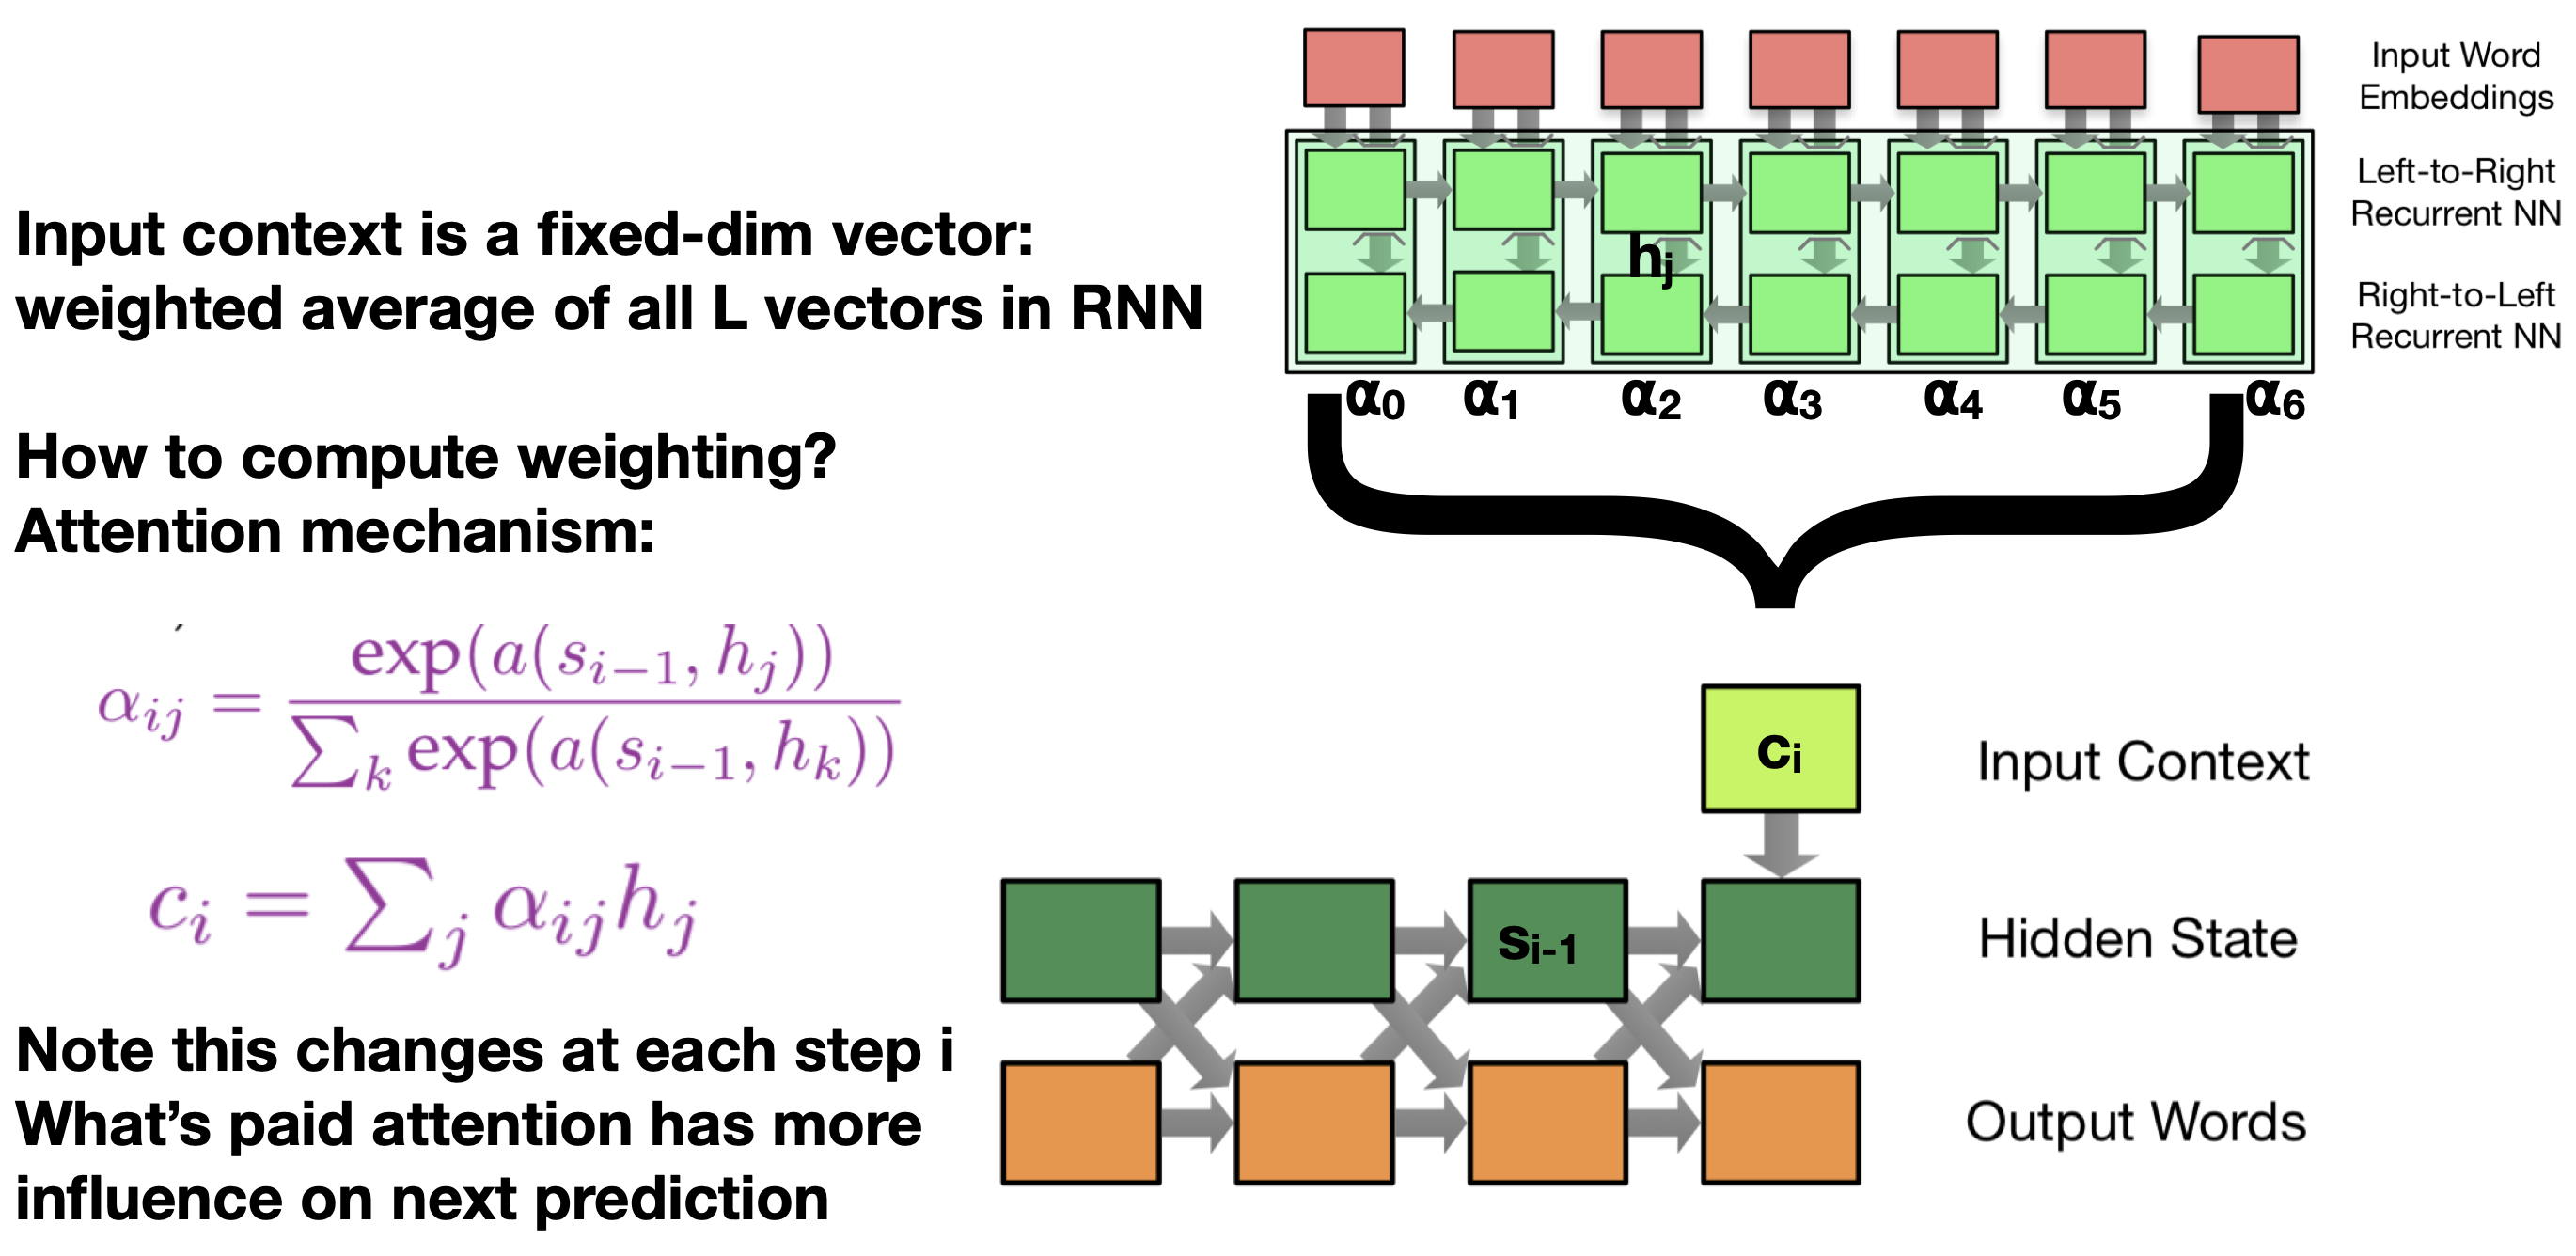
\includegraphics[scale=0.3]{first-midterm-2025/mt-rnn.png}
\end{center}
\begin{enumerate}

\item What would happen to the Machine Translation (MT) system output if the input context $c_i$ is removed or set to zero? 
\hfill{\em (4 points)}
\solution{The MT system will not be using any input information from the encoder. It might just hallucinate and not translate.}{\vspace{4cm}}

\item Explain what is the intuition behind $\alpha_{ij}$ in the equation $c_i = \sum_j \alpha_{ij} h_j$? 
\hfill{\em (4 points)}
\solution{$\alpha_{ij}$ represents the relevance/importance of input word at position $j$ for the decoding step $i$. Words with high $\alpha_{ij}$ will be emphasized in weighted average $c_i$ and therefore will impact the decoding of the next word.}{\vspace{4cm}}

\item Suppose we replaced all $h_j$ (contextual embedding) in the $\alpha_{ij}$ and $c_i$ equations with the input word embeddings instead. What do you think will happen? 
\hfill{\em (2 points)}
\solution{All reasonable answers will be accepted. For example: The MT system might still work since we are still giving it word embeddings, but it might perform worse since the embeddings are static. Alternative example: The MT system will fail because it can no longer contextual embeddings are extremely important. Yet another example: Transformers do not use RNN encoders, so maybe it will be ok given sufficient training.}{\vspace{5cm}}

\end{enumerate}

\newpage
\section*{Extra Space}
\newpage
\end{document}

